%
\begin{isabellebody}%
\def\isabellecontext{Typedefs}%
%
\isadelimtheory
%
\endisadelimtheory
%
\isatagtheory
%
\endisatagtheory
{\isafoldtheory}%
%
\isadelimtheory
%
\endisadelimtheory
%
\isamarkupsection{Introducing New Types%
}
\isamarkuptrue%
%
\begin{isamarkuptext}%
\label{sec:adv-typedef}
For most applications, a combination of predefined types like \isa{bool} and
\isa{{\isaliteral{5C3C52696768746172726F773E}{\isasymRightarrow}}} with recursive datatypes and records is quite sufficient. Very
occasionally you may feel the need for a more advanced type.  If you
are certain that your type is not definable by any of the
standard means, then read on.
\begin{warn}
  Types in HOL must be non-empty; otherwise the quantifier rules would be
  unsound, because $\exists x.\ x=x$ is a theorem.
\end{warn}%
\end{isamarkuptext}%
\isamarkuptrue%
%
\isamarkupsubsection{Declaring New Types%
}
\isamarkuptrue%
%
\begin{isamarkuptext}%
\label{sec:typedecl}
\index{types!declaring|(}%
\index{typedecl@\isacommand {typedecl} (command)}%
The most trivial way of introducing a new type is by a \textbf{type
declaration}:%
\end{isamarkuptext}%
\isamarkuptrue%
\isacommand{typedecl}\isamarkupfalse%
\ my{\isaliteral{5F}{\isacharunderscore}}new{\isaliteral{5F}{\isacharunderscore}}type%
\begin{isamarkuptext}%
\noindent
This does not define \isa{my{\isaliteral{5F}{\isacharunderscore}}new{\isaliteral{5F}{\isacharunderscore}}type} at all but merely introduces its
name. Thus we know nothing about this type, except that it is
non-empty. Such declarations without definitions are
useful if that type can be viewed as a parameter of the theory.
A typical example is given in \S\ref{sec:VMC}, where we define a transition
relation over an arbitrary type of states.

In principle we can always get rid of such type declarations by making those
types parameters of every other type, thus keeping the theory generic. In
practice, however, the resulting clutter can make types hard to read.

If you are looking for a quick and dirty way of introducing a new type
together with its properties: declare the type and state its properties as
axioms. Example:%
\end{isamarkuptext}%
\isamarkuptrue%
\isacommand{axioms}\isamarkupfalse%
\isanewline
just{\isaliteral{5F}{\isacharunderscore}}one{\isaliteral{3A}{\isacharcolon}}\ {\isaliteral{22}{\isachardoublequoteopen}}{\isaliteral{5C3C6578697374733E}{\isasymexists}}x{\isaliteral{3A}{\isacharcolon}}{\isaliteral{3A}{\isacharcolon}}my{\isaliteral{5F}{\isacharunderscore}}new{\isaliteral{5F}{\isacharunderscore}}type{\isaliteral{2E}{\isachardot}}\ {\isaliteral{5C3C666F72616C6C3E}{\isasymforall}}y{\isaliteral{2E}{\isachardot}}\ x\ {\isaliteral{3D}{\isacharequal}}\ y{\isaliteral{22}{\isachardoublequoteclose}}%
\begin{isamarkuptext}%
\noindent
However, we strongly discourage this approach, except at explorative stages
of your development. It is extremely easy to write down contradictory sets of
axioms, in which case you will be able to prove everything but it will mean
nothing.  In the example above, the axiomatic approach is
unnecessary: a one-element type called \isa{unit} is already defined in HOL.
\index{types!declaring|)}%
\end{isamarkuptext}%
\isamarkuptrue%
%
\isamarkupsubsection{Defining New Types%
}
\isamarkuptrue%
%
\begin{isamarkuptext}%
\label{sec:typedef}
\index{types!defining|(}%
\index{typedecl@\isacommand {typedef} (command)|(}%
Now we come to the most general means of safely introducing a new type, the
\textbf{type definition}. All other means, for example
\isacommand{datatype}, are based on it. The principle is extremely simple:
any non-empty subset of an existing type can be turned into a new type.
More precisely, the new type is specified to be isomorphic to some
non-empty subset of an existing type.

Let us work a simple example, the definition of a three-element type.
It is easily represented by the first three natural numbers:%
\end{isamarkuptext}%
\isamarkuptrue%
\isacommand{typedef}\isamarkupfalse%
\ three\ {\isaliteral{3D}{\isacharequal}}\ {\isaliteral{22}{\isachardoublequoteopen}}{\isaliteral{7B}{\isacharbraceleft}}{\isadigit{0}}{\isaliteral{3A}{\isacharcolon}}{\isaliteral{3A}{\isacharcolon}}nat{\isaliteral{2C}{\isacharcomma}}\ {\isadigit{1}}{\isaliteral{2C}{\isacharcomma}}\ {\isadigit{2}}{\isaliteral{7D}{\isacharbraceright}}{\isaliteral{22}{\isachardoublequoteclose}}%
\isadelimproof
%
\endisadelimproof
%
\isatagproof
%
\begin{isamarkuptxt}%
\noindent
In order to enforce that the representing set on the right-hand side is
non-empty, this definition actually starts a proof to that effect:
\begin{isabelle}%
\ {\isadigit{1}}{\isaliteral{2E}{\isachardot}}\ {\isaliteral{5C3C6578697374733E}{\isasymexists}}x{\isaliteral{2E}{\isachardot}}\ x\ {\isaliteral{5C3C696E3E}{\isasymin}}\ {\isaliteral{7B}{\isacharbraceleft}}{\isadigit{0}}{\isaliteral{2C}{\isacharcomma}}\ {\isadigit{1}}{\isaliteral{2C}{\isacharcomma}}\ {\isadigit{2}}{\isaliteral{7D}{\isacharbraceright}}%
\end{isabelle}
Fortunately, this is easy enough to show, even \isa{auto} could do it.
In general, one has to provide a witness, in our case 0:%
\end{isamarkuptxt}%
\isamarkuptrue%
\isacommand{apply}\isamarkupfalse%
{\isaliteral{28}{\isacharparenleft}}rule{\isaliteral{5F}{\isacharunderscore}}tac\ x\ {\isaliteral{3D}{\isacharequal}}\ {\isadigit{0}}\ \isakeyword{in}\ exI{\isaliteral{29}{\isacharparenright}}\isanewline
\isacommand{by}\isamarkupfalse%
\ simp%
\endisatagproof
{\isafoldproof}%
%
\isadelimproof
%
\endisadelimproof
%
\begin{isamarkuptext}%
This type definition introduces the new type \isa{three} and asserts
that it is a copy of the set \isa{{\isaliteral{7B}{\isacharbraceleft}}{\isadigit{0}}{\isaliteral{2C}{\isacharcomma}}\ {\isadigit{1}}{\isaliteral{2C}{\isacharcomma}}\ {\isadigit{2}}{\isaliteral{7D}{\isacharbraceright}}}. This assertion
is expressed via a bijection between the \emph{type} \isa{three} and the
\emph{set} \isa{{\isaliteral{7B}{\isacharbraceleft}}{\isadigit{0}}{\isaliteral{2C}{\isacharcomma}}\ {\isadigit{1}}{\isaliteral{2C}{\isacharcomma}}\ {\isadigit{2}}{\isaliteral{7D}{\isacharbraceright}}}. To this end, the command declares the following
constants behind the scenes:
\begin{center}
\begin{tabular}{rcl}
\isa{three} &::& \isa{nat\ set} \\
\isa{Rep{\isaliteral{5F}{\isacharunderscore}}three} &::& \isa{three\ {\isaliteral{5C3C52696768746172726F773E}{\isasymRightarrow}}\ nat}\\
\isa{Abs{\isaliteral{5F}{\isacharunderscore}}three} &::& \isa{nat\ {\isaliteral{5C3C52696768746172726F773E}{\isasymRightarrow}}\ three}
\end{tabular}
\end{center}
where constant \isa{three} is explicitly defined as the representing set:
\begin{center}
\isa{three\ {\isaliteral{5C3C65717569763E}{\isasymequiv}}\ {\isaliteral{7B}{\isacharbraceleft}}{\isadigit{0}}{\isaliteral{2C}{\isacharcomma}}\ {\isadigit{1}}{\isaliteral{2C}{\isacharcomma}}\ {\isadigit{2}}{\isaliteral{7D}{\isacharbraceright}}}\hfill(\isa{three{\isaliteral{5F}{\isacharunderscore}}def})
\end{center}
The situation is best summarized with the help of the following diagram,
where squares denote types and the irregular region denotes a set:
\begin{center}
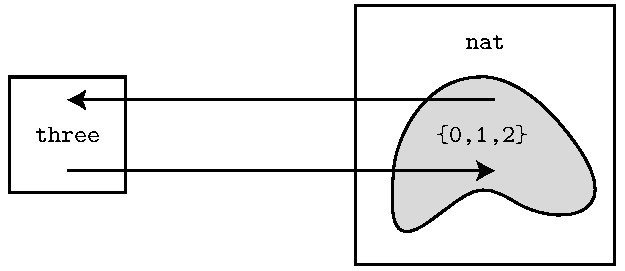
\includegraphics[scale=.8]{typedef}
\end{center}
Finally, \isacommand{typedef} asserts that \isa{Rep{\isaliteral{5F}{\isacharunderscore}}three} is
surjective on the subset \isa{three} and \isa{Abs{\isaliteral{5F}{\isacharunderscore}}three} and \isa{Rep{\isaliteral{5F}{\isacharunderscore}}three} are inverses of each other:
\begin{center}
\begin{tabular}{@ {}r@ {\qquad\qquad}l@ {}}
\isa{Rep{\isaliteral{5F}{\isacharunderscore}}three\ x\ {\isaliteral{5C3C696E3E}{\isasymin}}\ three} & (\isa{Rep{\isaliteral{5F}{\isacharunderscore}}three}) \\
\isa{Abs{\isaliteral{5F}{\isacharunderscore}}three\ {\isaliteral{28}{\isacharparenleft}}Rep{\isaliteral{5F}{\isacharunderscore}}three\ x{\isaliteral{29}{\isacharparenright}}\ {\isaliteral{3D}{\isacharequal}}\ x} & (\isa{Rep{\isaliteral{5F}{\isacharunderscore}}three{\isaliteral{5F}{\isacharunderscore}}inverse}) \\
\isa{y\ {\isaliteral{5C3C696E3E}{\isasymin}}\ three\ {\isaliteral{5C3C4C6F6E6772696768746172726F773E}{\isasymLongrightarrow}}\ Rep{\isaliteral{5F}{\isacharunderscore}}three\ {\isaliteral{28}{\isacharparenleft}}Abs{\isaliteral{5F}{\isacharunderscore}}three\ y{\isaliteral{29}{\isacharparenright}}\ {\isaliteral{3D}{\isacharequal}}\ y} & (\isa{Abs{\isaliteral{5F}{\isacharunderscore}}three{\isaliteral{5F}{\isacharunderscore}}inverse})
\end{tabular}
\end{center}
%
From this example it should be clear what \isacommand{typedef} does
in general given a name (here \isa{three}) and a set
(here \isa{{\isaliteral{7B}{\isacharbraceleft}}{\isadigit{0}}{\isaliteral{2C}{\isacharcomma}}\ {\isadigit{1}}{\isaliteral{2C}{\isacharcomma}}\ {\isadigit{2}}{\isaliteral{7D}{\isacharbraceright}}}).

Our next step is to define the basic functions expected on the new type.
Although this depends on the type at hand, the following strategy works well:
\begin{itemize}
\item define a small kernel of basic functions that can express all other
functions you anticipate.
\item define the kernel in terms of corresponding functions on the
representing type using \isa{Abs} and \isa{Rep} to convert between the
two levels.
\end{itemize}
In our example it suffices to give the three elements of type \isa{three}
names:%
\end{isamarkuptext}%
\isamarkuptrue%
\isacommand{definition}\isamarkupfalse%
\ A\ {\isaliteral{3A}{\isacharcolon}}{\isaliteral{3A}{\isacharcolon}}\ three\ \isakeyword{where}\ {\isaliteral{22}{\isachardoublequoteopen}}A\ {\isaliteral{5C3C65717569763E}{\isasymequiv}}\ Abs{\isaliteral{5F}{\isacharunderscore}}three\ {\isadigit{0}}{\isaliteral{22}{\isachardoublequoteclose}}\isanewline
\isacommand{definition}\isamarkupfalse%
\ B\ {\isaliteral{3A}{\isacharcolon}}{\isaliteral{3A}{\isacharcolon}}\ three\ \isakeyword{where}\ {\isaliteral{22}{\isachardoublequoteopen}}B\ {\isaliteral{5C3C65717569763E}{\isasymequiv}}\ Abs{\isaliteral{5F}{\isacharunderscore}}three\ {\isadigit{1}}{\isaliteral{22}{\isachardoublequoteclose}}\isanewline
\isacommand{definition}\isamarkupfalse%
\ C\ {\isaliteral{3A}{\isacharcolon}}{\isaliteral{3A}{\isacharcolon}}\ three\ \isakeyword{where}\ {\isaliteral{22}{\isachardoublequoteopen}}C\ {\isaliteral{5C3C65717569763E}{\isasymequiv}}\ Abs{\isaliteral{5F}{\isacharunderscore}}three\ {\isadigit{2}}{\isaliteral{22}{\isachardoublequoteclose}}%
\begin{isamarkuptext}%
So far, everything was easy. But it is clear that reasoning about \isa{three} will be hell if we have to go back to \isa{nat} every time. Thus our
aim must be to raise our level of abstraction by deriving enough theorems
about type \isa{three} to characterize it completely. And those theorems
should be phrased in terms of \isa{A}, \isa{B} and \isa{C}, not \isa{Abs{\isaliteral{5F}{\isacharunderscore}}three} and \isa{Rep{\isaliteral{5F}{\isacharunderscore}}three}. Because of the simplicity of the example,
we merely need to prove that \isa{A}, \isa{B} and \isa{C} are distinct
and that they exhaust the type.

In processing our \isacommand{typedef} declaration, 
Isabelle proves several helpful lemmas. The first two
express injectivity of \isa{Rep{\isaliteral{5F}{\isacharunderscore}}three} and \isa{Abs{\isaliteral{5F}{\isacharunderscore}}three}:
\begin{center}
\begin{tabular}{@ {}r@ {\qquad}l@ {}}
\isa{{\isaliteral{28}{\isacharparenleft}}Rep{\isaliteral{5F}{\isacharunderscore}}three\ x\ {\isaliteral{3D}{\isacharequal}}\ Rep{\isaliteral{5F}{\isacharunderscore}}three\ y{\isaliteral{29}{\isacharparenright}}\ {\isaliteral{3D}{\isacharequal}}\ {\isaliteral{28}{\isacharparenleft}}x\ {\isaliteral{3D}{\isacharequal}}\ y{\isaliteral{29}{\isacharparenright}}} & (\isa{Rep{\isaliteral{5F}{\isacharunderscore}}three{\isaliteral{5F}{\isacharunderscore}}inject}) \\
\begin{tabular}{@ {}l@ {}}
\isa{{\isaliteral{5C3C6C6272616B6B3E}{\isasymlbrakk}}x\ {\isaliteral{5C3C696E3E}{\isasymin}}\ three{\isaliteral{3B}{\isacharsemicolon}}\ y\ {\isaliteral{5C3C696E3E}{\isasymin}}\ three\ {\isaliteral{5C3C726272616B6B3E}{\isasymrbrakk}}} \\
\isa{{\isaliteral{5C3C4C6F6E6772696768746172726F773E}{\isasymLongrightarrow}}\ {\isaliteral{28}{\isacharparenleft}}Abs{\isaliteral{5F}{\isacharunderscore}}three\ x\ {\isaliteral{3D}{\isacharequal}}\ Abs{\isaliteral{5F}{\isacharunderscore}}three\ y{\isaliteral{29}{\isacharparenright}}\ {\isaliteral{3D}{\isacharequal}}\ {\isaliteral{28}{\isacharparenleft}}x\ {\isaliteral{3D}{\isacharequal}}\ y{\isaliteral{29}{\isacharparenright}}}
\end{tabular} & (\isa{Abs{\isaliteral{5F}{\isacharunderscore}}three{\isaliteral{5F}{\isacharunderscore}}inject}) \\
\end{tabular}
\end{center}
The following ones allow to replace some \isa{x{\isaliteral{3A}{\isacharcolon}}{\isaliteral{3A}{\isacharcolon}}three} by
\isa{Abs{\isaliteral{5F}{\isacharunderscore}}three{\isaliteral{28}{\isacharparenleft}}y{\isaliteral{3A}{\isacharcolon}}{\isaliteral{3A}{\isacharcolon}}nat{\isaliteral{29}{\isacharparenright}}}, and conversely \isa{y} by \isa{Rep{\isaliteral{5F}{\isacharunderscore}}three\ x}:
\begin{center}
\begin{tabular}{@ {}r@ {\qquad}l@ {}}
\isa{{\isaliteral{5C3C6C6272616B6B3E}{\isasymlbrakk}}y\ {\isaliteral{5C3C696E3E}{\isasymin}}\ three{\isaliteral{3B}{\isacharsemicolon}}\ {\isaliteral{5C3C416E643E}{\isasymAnd}}x{\isaliteral{2E}{\isachardot}}\ y\ {\isaliteral{3D}{\isacharequal}}\ Rep{\isaliteral{5F}{\isacharunderscore}}three\ x\ {\isaliteral{5C3C4C6F6E6772696768746172726F773E}{\isasymLongrightarrow}}\ P{\isaliteral{5C3C726272616B6B3E}{\isasymrbrakk}}\ {\isaliteral{5C3C4C6F6E6772696768746172726F773E}{\isasymLongrightarrow}}\ P} & (\isa{Rep{\isaliteral{5F}{\isacharunderscore}}three{\isaliteral{5F}{\isacharunderscore}}cases}) \\
\isa{{\isaliteral{28}{\isacharparenleft}}{\isaliteral{5C3C416E643E}{\isasymAnd}}y{\isaliteral{2E}{\isachardot}}\ {\isaliteral{5C3C6C6272616B6B3E}{\isasymlbrakk}}x\ {\isaliteral{3D}{\isacharequal}}\ Abs{\isaliteral{5F}{\isacharunderscore}}three\ y{\isaliteral{3B}{\isacharsemicolon}}\ y\ {\isaliteral{5C3C696E3E}{\isasymin}}\ three{\isaliteral{5C3C726272616B6B3E}{\isasymrbrakk}}\ {\isaliteral{5C3C4C6F6E6772696768746172726F773E}{\isasymLongrightarrow}}\ P{\isaliteral{29}{\isacharparenright}}\ {\isaliteral{5C3C4C6F6E6772696768746172726F773E}{\isasymLongrightarrow}}\ P} & (\isa{Abs{\isaliteral{5F}{\isacharunderscore}}three{\isaliteral{5F}{\isacharunderscore}}cases}) \\
\isa{{\isaliteral{5C3C6C6272616B6B3E}{\isasymlbrakk}}y\ {\isaliteral{5C3C696E3E}{\isasymin}}\ three{\isaliteral{3B}{\isacharsemicolon}}\ {\isaliteral{5C3C416E643E}{\isasymAnd}}x{\isaliteral{2E}{\isachardot}}\ P\ {\isaliteral{28}{\isacharparenleft}}Rep{\isaliteral{5F}{\isacharunderscore}}three\ x{\isaliteral{29}{\isacharparenright}}{\isaliteral{5C3C726272616B6B3E}{\isasymrbrakk}}\ {\isaliteral{5C3C4C6F6E6772696768746172726F773E}{\isasymLongrightarrow}}\ P\ y} & (\isa{Rep{\isaliteral{5F}{\isacharunderscore}}three{\isaliteral{5F}{\isacharunderscore}}induct}) \\
\isa{{\isaliteral{28}{\isacharparenleft}}{\isaliteral{5C3C416E643E}{\isasymAnd}}y{\isaliteral{2E}{\isachardot}}\ y\ {\isaliteral{5C3C696E3E}{\isasymin}}\ three\ {\isaliteral{5C3C4C6F6E6772696768746172726F773E}{\isasymLongrightarrow}}\ P\ {\isaliteral{28}{\isacharparenleft}}Abs{\isaliteral{5F}{\isacharunderscore}}three\ y{\isaliteral{29}{\isacharparenright}}{\isaliteral{29}{\isacharparenright}}\ {\isaliteral{5C3C4C6F6E6772696768746172726F773E}{\isasymLongrightarrow}}\ P\ x} & (\isa{Abs{\isaliteral{5F}{\isacharunderscore}}three{\isaliteral{5F}{\isacharunderscore}}induct}) \\
\end{tabular}
\end{center}
These theorems are proved for any type definition, with \isa{three}
replaced by the name of the type in question.

Distinctness of \isa{A}, \isa{B} and \isa{C} follows immediately
if we expand their definitions and rewrite with the injectivity
of \isa{Abs{\isaliteral{5F}{\isacharunderscore}}three}:%
\end{isamarkuptext}%
\isamarkuptrue%
\isacommand{lemma}\isamarkupfalse%
\ {\isaliteral{22}{\isachardoublequoteopen}}A\ {\isaliteral{5C3C6E6F7465713E}{\isasymnoteq}}\ B\ {\isaliteral{5C3C616E643E}{\isasymand}}\ B\ {\isaliteral{5C3C6E6F7465713E}{\isasymnoteq}}\ A\ {\isaliteral{5C3C616E643E}{\isasymand}}\ A\ {\isaliteral{5C3C6E6F7465713E}{\isasymnoteq}}\ C\ {\isaliteral{5C3C616E643E}{\isasymand}}\ C\ {\isaliteral{5C3C6E6F7465713E}{\isasymnoteq}}\ A\ {\isaliteral{5C3C616E643E}{\isasymand}}\ B\ {\isaliteral{5C3C6E6F7465713E}{\isasymnoteq}}\ C\ {\isaliteral{5C3C616E643E}{\isasymand}}\ C\ {\isaliteral{5C3C6E6F7465713E}{\isasymnoteq}}\ B{\isaliteral{22}{\isachardoublequoteclose}}\isanewline
%
\isadelimproof
%
\endisadelimproof
%
\isatagproof
\isacommand{by}\isamarkupfalse%
{\isaliteral{28}{\isacharparenleft}}simp\ add{\isaliteral{3A}{\isacharcolon}}\ Abs{\isaliteral{5F}{\isacharunderscore}}three{\isaliteral{5F}{\isacharunderscore}}inject\ A{\isaliteral{5F}{\isacharunderscore}}def\ B{\isaliteral{5F}{\isacharunderscore}}def\ C{\isaliteral{5F}{\isacharunderscore}}def\ three{\isaliteral{5F}{\isacharunderscore}}def{\isaliteral{29}{\isacharparenright}}%
\endisatagproof
{\isafoldproof}%
%
\isadelimproof
%
\endisadelimproof
%
\begin{isamarkuptext}%
\noindent
Of course we rely on the simplifier to solve goals like \isa{{\isadigit{0}}\ {\isaliteral{5C3C6E6F7465713E}{\isasymnoteq}}\ {\isadigit{1}}}.

The fact that \isa{A}, \isa{B} and \isa{C} exhaust type \isa{three} is
best phrased as a case distinction theorem: if you want to prove \isa{P\ x}
(where \isa{x} is of type \isa{three}) it suffices to prove \isa{P\ A},
\isa{P\ B} and \isa{P\ C}:%
\end{isamarkuptext}%
\isamarkuptrue%
\isacommand{lemma}\isamarkupfalse%
\ three{\isaliteral{5F}{\isacharunderscore}}cases{\isaliteral{3A}{\isacharcolon}}\ {\isaliteral{22}{\isachardoublequoteopen}}{\isaliteral{5C3C6C6272616B6B3E}{\isasymlbrakk}}\ P\ A{\isaliteral{3B}{\isacharsemicolon}}\ P\ B{\isaliteral{3B}{\isacharsemicolon}}\ P\ C\ {\isaliteral{5C3C726272616B6B3E}{\isasymrbrakk}}\ {\isaliteral{5C3C4C6F6E6772696768746172726F773E}{\isasymLongrightarrow}}\ P\ x{\isaliteral{22}{\isachardoublequoteclose}}%
\isadelimproof
%
\endisadelimproof
%
\isatagproof
%
\begin{isamarkuptxt}%
\noindent Again this follows easily using the induction principle stemming from the type definition:%
\end{isamarkuptxt}%
\isamarkuptrue%
\isacommand{apply}\isamarkupfalse%
{\isaliteral{28}{\isacharparenleft}}induct{\isaliteral{5F}{\isacharunderscore}}tac\ x{\isaliteral{29}{\isacharparenright}}%
\begin{isamarkuptxt}%
\begin{isabelle}%
\ {\isadigit{1}}{\isaliteral{2E}{\isachardot}}\ {\isaliteral{5C3C416E643E}{\isasymAnd}}y{\isaliteral{2E}{\isachardot}}\ {\isaliteral{5C3C6C6272616B6B3E}{\isasymlbrakk}}P\ A{\isaliteral{3B}{\isacharsemicolon}}\ P\ B{\isaliteral{3B}{\isacharsemicolon}}\ P\ C{\isaliteral{3B}{\isacharsemicolon}}\ y\ {\isaliteral{5C3C696E3E}{\isasymin}}\ three{\isaliteral{5C3C726272616B6B3E}{\isasymrbrakk}}\ {\isaliteral{5C3C4C6F6E6772696768746172726F773E}{\isasymLongrightarrow}}\ P\ {\isaliteral{28}{\isacharparenleft}}Abs{\isaliteral{5F}{\isacharunderscore}}three\ y{\isaliteral{29}{\isacharparenright}}%
\end{isabelle}
Simplification with \isa{three{\isaliteral{5F}{\isacharunderscore}}def} leads to the disjunction \isa{y\ {\isaliteral{3D}{\isacharequal}}\ {\isadigit{0}}\ {\isaliteral{5C3C6F723E}{\isasymor}}\ y\ {\isaliteral{3D}{\isacharequal}}\ {\isadigit{1}}\ {\isaliteral{5C3C6F723E}{\isasymor}}\ y\ {\isaliteral{3D}{\isacharequal}}\ {\isadigit{2}}} which \isa{auto} separates into three
subgoals, each of which is easily solved by simplification:%
\end{isamarkuptxt}%
\isamarkuptrue%
\isacommand{apply}\isamarkupfalse%
{\isaliteral{28}{\isacharparenleft}}auto\ simp\ add{\isaliteral{3A}{\isacharcolon}}\ three{\isaliteral{5F}{\isacharunderscore}}def\ A{\isaliteral{5F}{\isacharunderscore}}def\ B{\isaliteral{5F}{\isacharunderscore}}def\ C{\isaliteral{5F}{\isacharunderscore}}def{\isaliteral{29}{\isacharparenright}}\isanewline
\isacommand{done}\isamarkupfalse%
%
\endisatagproof
{\isafoldproof}%
%
\isadelimproof
%
\endisadelimproof
%
\begin{isamarkuptext}%
\noindent
This concludes the derivation of the characteristic theorems for
type \isa{three}.

The attentive reader has realized long ago that the
above lengthy definition can be collapsed into one line:%
\end{isamarkuptext}%
\isamarkuptrue%
\isacommand{datatype}\isamarkupfalse%
\ better{\isaliteral{5F}{\isacharunderscore}}three\ {\isaliteral{3D}{\isacharequal}}\ A\ {\isaliteral{7C}{\isacharbar}}\ B\ {\isaliteral{7C}{\isacharbar}}\ C%
\begin{isamarkuptext}%
\noindent
In fact, the \isacommand{datatype} command performs internally more or less
the same derivations as we did, which gives you some idea what life would be
like without \isacommand{datatype}.

Although \isa{three} could be defined in one line, we have chosen this
example to demonstrate \isacommand{typedef} because its simplicity makes the
key concepts particularly easy to grasp. If you would like to see a
non-trivial example that cannot be defined more directly, we recommend the
definition of \emph{finite multisets} in the Library~\cite{HOL-Library}.

Let us conclude by summarizing the above procedure for defining a new type.
Given some abstract axiomatic description $P$ of a type $ty$ in terms of a
set of functions $F$, this involves three steps:
\begin{enumerate}
\item Find an appropriate type $\tau$ and subset $A$ which has the desired
  properties $P$, and make a type definition based on this representation.
\item Define the required functions $F$ on $ty$ by lifting
analogous functions on the representation via $Abs_ty$ and $Rep_ty$.
\item Prove that $P$ holds for $ty$ by lifting $P$ from the representation.
\end{enumerate}
You can now forget about the representation and work solely in terms of the
abstract functions $F$ and properties $P$.%
\index{typedecl@\isacommand {typedef} (command)|)}%
\index{types!defining|)}%
\end{isamarkuptext}%
\isamarkuptrue%
%
\isadelimtheory
%
\endisadelimtheory
%
\isatagtheory
%
\endisatagtheory
{\isafoldtheory}%
%
\isadelimtheory
%
\endisadelimtheory
\end{isabellebody}%
%%% Local Variables:
%%% mode: latex
%%% TeX-master: "root"
%%% End:
